% !TeX spellcheck = en_US
\section{Evaluating the Video Composition}
\label{690:Evaluating_Composition}
This section describes the evaluation of the semi-automatic CrowdCompose and the automatic AutoCompose.
Both approaches are discussed regarding the achieved quality of the video compositions, using subjective studies.

Finally, the performance of the contributions discussed in earlier chapters towards the video composition scenario is shown.
The quality assessment using the \ac{PaSC} and \ac{LiViU} are discussed in Section~\ref{sec:690_SupportiveApplications}.
\subsection{Experimental Setup}
The experiments performed for CrowdCompose and AutoCompose rely on the recording of five small- to mid-scale live events in 2014 in Singapore and Germany. 
Events E1 and E2 are used for evaluating parameter settings used in CrowdCompose.
E3, E4, and E5 are the bases for evaluating the composition quality of both CrowdCompose and AutoCompose. 
\subsubsection{CrowdCompose Users}
Details of the users recording video and taking part in the composition on CrowdCompose are given in Table~\ref{tab:690_demographics}.
Prepared recording devices using \ac{LiViU} are used for streaming. 
Devices are either the LG Nexus 4, LG Nexus 5 or OnePlus One smartphones. 
Training was conducted right before the events, and included a description of the event and how to use \ac{LiViU}.
Users are allowed to select the recording position freely and to move as they desire. 
A common scene, e.g., the playing field of a soccer game, is given for orientation.

During the evaluation, up to 30 concurrent workers on each CrowdCompose server instance are permitted. 
Three composition servers and one registration server are used.
In the evaluation section - unless stated otherwise - 10 minutes of the events E1 and E2 and 20 minutes of the events E3, E4, and E5 are evaluated. 
\begin{table}
	\centering 
	\caption{Evaluation statistics for CrowdCompose and AutoCompose.}
	\begin{tabular}{lcccccc}
		\toprule
		&\multicolumn{3}{c}{LiViU}  &\multicolumn{3}{c}{CrowdCompose} \\
		&No. & Age & \specialcell{Male\\Users}  & No.& Age  & \specialcell{Male\\Users}  \\ 
		\hline 
		\multicolumn{2}{c}{\textbf{Parameters}}\\
		E1-Sports & 4 & 20-28 & 4 & 46 & 16-42& 36\\
		E2-City& 7 & 19-32 & 7 & 72 & 18-51 & 58 \\
		\hline
		\multicolumn{2}{c}{\textbf{Evaluation}}\\
		E3-Music & 8 & 18-35 & 6 & 247 & 16-58 & 218 \\ 
		E4-Sports& 12 & 20-32 & 10 & 277 & 17-55 & 233   \\
		E5-News & 10  & 20-38 & 8 & 183 & 18-51 & 158  \\ 
		\bottomrule
	\end{tabular} 
	\label{tab:690_demographics}
\end{table}
The statistical data for workers in CrowdCompose is given in Table \ref{tab:690_demographics}. 
Additionally, the geographic region of the workers is included: 46.29\% have their origin in Asia, 39.9\% in Europe and 8.7\% from North America. 
The remaining share is distributed over the rest of the world.
Training of CrowdCompose workers is standardized by both a tutorial and a qualification task, as described in Section \ref{sec:620_reliability}. 
Training included the description, testing of the tools, and the explanation of the payment scheme of "punishments" and bonus.

\subsubsection{Videos}
The recordings from event E1 last 12:23 minutes; for E2 13:45 minutes. 
Event E1 records different sports activities at the central university sports day from different perspectives. 
The event E2 is a tour in Darmstadt, Germany, showing \ac{PoI}s and explanations by a guide. 
The evaluation video dataset includes recordings from a regional soccer stadium (26:59 minutes), a regional Music Festival (23:39 minutes) and the University Festival Report (22:33 minutes). 
The university festival report shows the annual celebration of the school. 
A speaker acts as a guide throughout the video, and diverse recordings are made - ranging from a stage including musicians to speeches by faculty members as well as an art exhibition.
\subsubsection{Questions Discussed in this Evaluation}

Central questions in the evaluation of CrowdCompose are:
\begin{enumerate}
	\item How can the parameters of CrowdCompose be set to allow workers make reliable assessments?
	\item How much delay between the composition and the live event is needed for a good composition?
	\item Which perceived quality does CrowdCompose achieve in comparison to automatic composition algorithms?
	\item Can a sufficient worker pool be established to timely compose video?
\end{enumerate}
From the composed video streams, AutoCompose learns how to compose a video.
The central research question for AutoCompose is if the composed video streams achieve a superior quality in comparison with existing automatic composition algorithms.
\subsection{Parameter Study}
\label{sec:690_eval_crowdcompose}
The first question for evaluating CrowdCompose addresses the optimal configuration to achieve a trade-off between the "liveness" of the composition and reliable assessments.
CrowdCompose uses two parameters that need to be discussed: the length of a round $t_{r}$ and the number of parallel rounds $n$. 

\subsubsection{Broadcast Delay}
Both parameters have an influence on the broadcast delay.
A high broadcast delay affects the composed video's perceived quality. 
Artificial delays are technically required and common in today's broadcasting environment.

To understand which delay is acceptable, an experiment with 33 assessors mediated over the crowdsourcing platform Microworkers\footnote{www.microworkers.com; Visited on: 09/02/2016} is set up.
Different video genres are selected for the composition ranging from sports, news and music.  
A web page that includes a live newsfeed  illustrating important events and a video being delayed by several seconds is shown. 
Users were asked to judge the impact of the delay on their viewing experience.

Sports broadcasts suffer immediately, as starting with delays of 20 seconds nearly the half of all viewers (43.1\%), and for 40 seconds 68.4\% of the viewers rated the delay as being distracting. 
Contrarily, for news broadcasts, more than half of the assessors accepted 30 seconds of delay or more.

The music performance was rated even less critical. 
For a majority of the assessors, a delay of 40 seconds was still acceptable. 
\ac{IP}TV broadcasters such as Magine.TV\footnote{www.magine.tv; Visited on: 10/06/2016} have a delay of 53 seconds for sports broadcasts\footnote{www.heise.de/newsticker/meldung/Zahlen-bitte-Euro-2016-Manche-jubeln-erst-nach-56-Sekunden-3228756.html; Visited on: 09/25/2016}.
CrowdCompose has to comply with the delay requirements.
CrowdCompose's task design can be adjusted to comply with the findings and achieve a guaranteed broadcast delay of 20 to 40 seconds by setting the values for $n$ and $t_{r}$ accordingly. 
\subsubsection{Reliability of the Assessment}
The second research question addresses the reliability of the judgment of the workers.
$t_{r}$ describes the round time, but additionally the time of the video segment which can be accessed by workers.
It is thus a time limit for allowing workers to judge the quality of different views.
Setting the value allows for complying with given subjective quality assessment rules (see ITU-R P.910)~\cite{ITU-J2008}.
Videos shall be shown for around 10 seconds to allow a reliable assessment of the quality.
 
$t_r$ is evaluated for 5, 10 and 15 seconds.
Table~\ref{tab:690_rating_time_consistency} shows the average required time for an assessor to complete Task 1a and the consistency on judgments for E1 and E2. 
The consistency of judgments defines the percentage of common judgments across all workers on the best video view.

For CrowdCompose a round time between 5 seconds and 10 seconds performs best. 
Whereas for E1 half of the workforce could complete the assessment in 6.8 seconds this took longer for E2 (8.3 seconds). 

For E1 the consistency is highest at $t_{r}=10$. In contrast to this, for E2 the system performs best at $t_{r}=5$.
Longer $t_{r}$ shows no improvement.
Depending on the genre of the video, the round time is chosen with 5 or 10 seconds, respectively. 
\begin{table}
	\centering 
	\caption[CrowdCompose: Rating time and consistency of judgments]{CrowdCompose: Rating time and consistency of judgments across workers. Consistency of judgments depicts how many users agreed on the same view. The system was evaluated with two video views.}
	\begin{tabular}{ccccc}
		\toprule
		& &\multicolumn{3}{c}{$t_{r}$}  \\
		& & 5s & 10s & 15s  \\ 
		\hline 
		\multirow{ 2}{*}{\specialcell{Rating time \\ Median $[s]$}}  & E1 & 6.8s & 13.1s & 14.9s \\ 
		& E2 & 8.3s & 10.9s & 15.3s \\ 
		\multirow{ 2}{*}{\specialcell{Consistency $[\%]$}}  & E1 & 59\% & 68\% & 67\% \\ 
		& E2 & 63\% & 54\% & 56\% \\ 
	\bottomrule
	\end{tabular} 
	\label{tab:690_rating_time_consistency}
\end{table}

The number of rounds $n$ determines how many video segments of a view are assessed in parallel.
An increase of $n$ - the number of parallel rounds - enhances the rating consistency. 
The consistency increases by 11\% until three parallel rounds. 

With more than three rounds no increase in the consistency of judgments could be observed. 
The broadcast delay is chosen as a constant, independent value for each genre.
Assessments of workers which require more than $n*t_{r}+b_c$ are discarded. 
The combination of $n*t_{r}$ is chosen to comply with $BD = n*t_{r} + b_c + 5$ being equal or less than the accepted delay for the genres music: $BD \leq 30$; sports: $BD \leq 20$ and news: $BD \leq 30$.  
It affects the overall broadcast delay. 
The feature was used in Task 2 at least once by 71.4\% of all workers.
If used, the average rewind time of workers is around 3.8 seconds. 
The parameter $b_c$ is set to 5 seconds for the system evaluation.
It allows workers to rewind the playback by 5 seconds.
\subsubsection{Assessing the Costs}
Workers cost money, so they should be wisely assigned to the individual tasks. 
The parameter $M$ defines the maximum number of workers assigned to a task. 
$M$ is a multiple of three. 
Table~\ref{tab:690_t2_refinement} shows the refinement tasks for view switches in Task 2 of CrowdCompose with different numbers of $M$ per refinement for the events E1 and E2. 
It can be observed that the refinement steps allow a rapid agreement on a three-second window for determining a video view switch. 
Second, an increase of workers takes longer to agree to the window at least for $M > 6$. 
Additionally, Task 2 converges after two to three refinements, even with a low number of workers completing. M = 6 is chosen for the remaining evaluation to obtain reliable results in a short amount of time.
\begin{table}
	\centering 
	\caption[CrowdCompose: Fraction of agreements in a three-second window]{CrowdCompose: Fraction of agreements in a three-second window ($\geq$50\% of the votes need to be in a window).}
	\begin{tabular}{ccccc}
		\toprule
		\multicolumn{2}{c}{$M$}& 3 & 6 & 9  \\ 
		\hline 
		\multirow{ 2}{*}{Initial Assessment}  & E1 & 7.9\% & 10.2\% & 3.9\% \\ 
		& E2 & 19\% & 18.3\% & 8.1\% \\ 
		\multirow{ 2}{*}{Refinement 1}  & E1 & 48\% & 54\% & 28.4\% \\ 
		& E2 & 31.1\% & 27.4\% & 24\% \\ 
		\multirow{ 2}{*}{Refinement 2}  & E1 & 39.6\% & 26.8\% & 38\% \\ 
		& E2 & 37.6\% & 45.4\% & 49.6\% \\
		\multirow{ 2}{*}{No window found}  & E1 & 4.5\% & 9\% & 29.7\% \\ 
		& E2 & 12.3\% & 8.9\% & 18.3\% \\
		\bottomrule
	\end{tabular} 
	\label{tab:690_t2_refinement}
\end{table}

\subsection{Perceived Quality of the Composed Video}
\label{sec:690_eval_perceived_quality}
Each of the composed videos is compared with automatic algorithms for composition \ac{AMGS}, MoviMash and the presentation of the single, best video view~\cite{Saini2012,Shrestha2010}.
The approach of Shrestha et al. optimizes the diversity of the shot selection and the overall quality using video quality assessment algorithms~\cite{Shrestha2010}.
For improving the quality, it leverages an objective quality metric.
In contrast to Shrestha et al.'s algorithm, MoviMash not only analyzes the video quality, but also introduces diversity regarding the recording position.
It is thus the most similar algorithm to CrowdCompose.
Both algorithms are described in Section~\ref{sec:240_videocomposition}.

Each event is assessed in a subjective quality study on the crowdsourcing platform Microworkers\footnote{www.microworkers.com; Visited on: 09/16/2016} by 35, 36 and 48 assessors\footnote{Reliability check excluded the assessments of 9 (E3), 3 (E4) and 7 (E5) users.}. 
From each composition, 60 seconds representing the same content are shown in random order.
The assessors are asked to judge the composition on an \ac{SSCQS}. 
The assessors do not know which composition algorithm created a video sequence.

\begin{figure}[!htb]
	\centering
	\subfloat[]{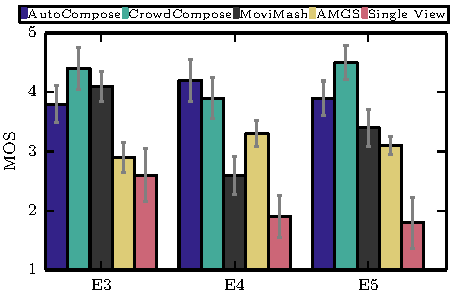
\includegraphics{./gfx/600_Composition/MOS_Composition}}
	\subfloat[]{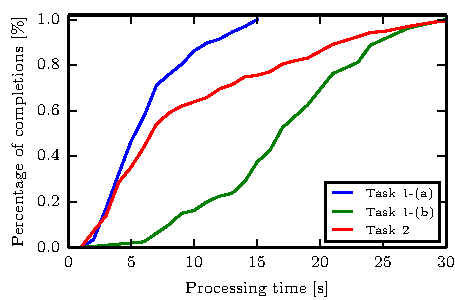
\includegraphics{./gfx/600_Composition/Response_time}}
	\caption[Evaluation results for CrowdCompose and AutoCompose]{Evaluation results for CrowdCompose and AutoCompose: (a) Evaluation of the perceived quality for compositions of events E3-E5. (b) Cumulative Distribution Function on the response times of workers for a 10 minute segment in event E4.}
	\label{fig:690_MOS}
\end{figure}
The results of this assessment are shown in Figure~\ref{fig:690_MOS} (a).
It depicts that the human composition and the proposed CrowdCompose outperform an automatic composition using \ac{AMGS}~\cite{Shrestha2010} and the presentation of a single view.
The improvements can be achieved as the CrowdCompose composition achieves a stable video quality comparable with the one of the \ac{AMGS} but places view switches better.
The diversity of the CrowdCompose composition is higher, and shot durations are more stable in comparison to the automatic algorithms. 
Considering the third research question, CrowdCompose generates a high quality video composition which is superior to existing automatic composition algorithms.

The accuracy of the video switch placement (Task 2) is discussed to understand if the placement and resulting shot durations are suitable.
A comparison with professionally produced content is made (see Table~\ref{tab:690_shots}). 
Ten professional live TV broadcasts from the two public German TV stations ARD and ZDF are used.
Shot lengths are determined in a manual annotation step. 
All recordings included video of more than 15 minutes and represented live footage of the genres "Entertainment," "News \& Talks" and "Sports".

In Table \ref{tab:690_shots} CrowdCompose achieves comparable shot durations but with a higher variance for news and music video. 
For professional sports broadcast the variance is higher compared to the composition of CrowdCompose, as, e.g., the minimum shot durations of 0.6 seconds cannot be achieved by CrowdCompose. 
The approach achieves the mean shot duration of "News \& Talks" and "Sports" live streams, but not of "Music" videos.
An explanation for the reduced average shot length in "Music" live streams is that even though they are streamed live, most of the show is scripted. 
The director thus knows in advance when to switch to which camera view.
In contrast to this, sports events have a higher uncertainty and thus can only be composed with a significant delay. 
Due to the three-second window in which the shot transition is determined, it is nearly impossible to achieve video shots of one-second length. 
An additional factor is that CrowdCompose generates outliers with long shot durations.
Especially for recordings close to the stage ("fr," "fc," and "fl") the manually determined shot durations are significantly higher than for those recorded at larger distances.
This finding goes in line with the findings on the recording position discussed in Chapter 3.

Nevertheless, the median of 7 seconds (genre: sports) shows that CrowdCompose is not yet able to ensure a timely composition for sports. 
For the remaining genres, the round time of ten seconds is a good choice.

\begin{table}[hb]
	\centering 
	\caption[Shot durations of composition approaches]{Shot durations in professionally edited live streams in comparison to CrowdCompose and AutoCompose.}
	\begin{tabular}{lccccccccc} 
		\toprule
		& \multicolumn{3}{c}{Professional} & \multicolumn{3}{c}{CrowdCompose} & \multicolumn{3}{c}{AutoCompose}\\
		\hline
		& Mean  & Median & Min & Mean  & Median & Min & Mean  & Median & Min\\
		\hline
		\textit{Sports} & 11.4s & 6.4s & 0.6s & 8.4s & 7s & 2s & 11.1s & 6s & 3s \\ 
		\textit{News} & 17.9s  & 13.9s & 1.1s & 13.6s & 12s & 3s & 15.9s & 8s & 3s\\ 
		\textit{Music}& 6.5s  & 5.7s & 1.1s & 7.1s & 6s & 2s  & 9.01s & 6s & 2s\\ 
		\bottomrule
	\end{tabular} 
	\label{tab:690_shots}
\end{table}

\subsection{Worker Task Times}
The response times for different task types in a real deployment of CrowdCompose are discussed now. 
For the event E4, a round time of five seconds at a total number of three rounds is chosen. 
As mentioned earlier, the broadcast delay is kept static over the complete broadcast. 
For the majority of workers, the successful completion of any task type is not a problem.
Most workers completed Task 1a in less than seven seconds. 
The more time-intensive task of assessing the different audio tracks (Task 1b) is less time-critical. 
Only a small fraction ($<$ 25\%) of workers require longer to complete. 
A majority of the workers complete the task successfully.

Task 2 also shows diverse response times. 
This is closely related to the refinement tasks. 
Workers of a first composition round watch the live stream and make their decision on a shot transition in a window of one second up to $\overline{D_{G}} + 2 \times \sigma D_{G}$.
As the window length is reduced, refinement decisions must be given in shorter times as the window length is reduced. 
\subsection{AutoCompose}
\label{sec:690_evalAutoCompose}
AutoCompose achieves a classification of a once trained composition model in real-time for the given models by leveraging content characteristics, a scene model and a filter stage that ensures cinematographic rules.
It learns the composition styles for placing shot boundaries and selects views by composition results presented by CrowdCompose.
The videos composed by AutoCompose are not part of the video set used to train the composition algorithm.

Events E3, E4 and E5 have been chosen to assess the performance of not only the CrowdCompose composition but also the AutoCompose composition. 
The resulting \ac{MOS} is depicted in Figure~\ref{fig:690_MOS} (a).
It shows that the AutoCompose composition achieves a similar quality for events E3, E4, and E5 in comparison to CrowdCompose, and it outperforms MoviMash~\cite{Saini2012} in one of three events.
At the same time and in contrast to MoviMash, AutoCompose conducts the composition in real-time.
Also, MoviMash suffers from a quality decrease if the genre of the video changes. 
MoviMash was developed for music recording compositions as in E4, but suffers from reduced quality in the remaining genres.

As the differences are not significant for some of the events a second, independent forced choice evaluation is performed.
Assessors are asked to compare two video sequences and to select the better one.
The focus lies on the compositions by AutoCompose, CrowdCompose, and MoviMash.
The sequences of 1) AutoCompose and CrowdCompose and 2) AutoCompose and MoviMash are compared.
As a subjective quality metric, \ac{JND} is chosen, as described in Section~\ref{sec:210_subjective_quality}.
The results show that CrowdCompose's composition is significantly better (JND $\geq 1$) for event E3 and E5, and slightly better for E4 (JND=0.31). 
Except for the composition of E3, AutoCompose shows a significant improvement in perception compared to MoviMash (JND $\geq 1$).
Thus, it can be concluded that the perceived quality is different for most genres and superior to the presentation of a single video view without quantifying the difference.
It is important to know that the results of forced choice experiments are not transitive; thus, it cannot be said that CrowdCompose achieves better results than MoviMash.

Furthermore, Table~\ref{tab:690_shots} depicts the resulting shot durations, which are in the case of AutoCompose different for each genre.
This is intended for AutoCompose.
AutoCompose's shot durations are slightly longer than those of the professional composition and the composition based on CrowdCompose.                                                                                                                                                                                               
\subsection{Supportive Applications}
\label{sec:690_SupportiveApplications}
During the setup of CrowdCompose and AutoCompose, the filter stage was used to eliminate poor quality video views.
An essential part of this stage is the usage of the scalable quality assessment algorithms and the \ac{PaSC}.
Furthermore, the delivery of video streams is achieved by using \ac{LiViU}.
\subsubsection{PaSC within the Video Composition}
For the \ac{PaSC} the video composition shows the real necessity for distributing quality assessment requests to mobile devices.
As a result, the number of parallel video streams and their encoding parameters (resolution, frame rate and bit rate) is heterogeneous. 
The number of videos being processed lies between 4 and 12.
The composition algorithm sets the deadline for processing requests. 

In comparison to the synthetic work traces evaluated in the evaluation of the \ac{PaSC} (see Section~\ref{556:Assessment_Eval}) the generated load on the devices and the server is lower.
The potential for leveraging resources of the mobile devices is still huge. 
Using the devices for quality assessment nearly doubled system utilization (measured in CPU load)  to around 28.3\% in comparison to a single server setup.
This allows the in-time processing of algorithms to be increased from around 68.8\% (single server) to an average of 93.22\%.
For any video composition application, the usage of a \ac{PaSC} system has the advantage of timely and more accurate quality assessments.
\subsubsection{LiViU in the Video Composition}
LiViU achieves the upload of video streams.
 Due to its design principles, if videos do not pass the checks for quality and compliance to cinematographic rules, the composition server can significantly reduce generated data traffic. As soon as a video view breaks the constraints of the filter stage, the video stream does not have to be submitted. In the aforementioned events E3 to E5, this achieves an average data traffic reduction by 23.9\%.
 